%!TEX root = ../CS263_project_report.tex

\section{Evaluation}
\label{sec:Eval}
\subsection{Profiling and Performance Considerations}
We profile the client execution on a large set of queries. Our profiling is mainly offline and allows us to assess the implementations' resource usage. The main profiling tool that we use is the Linux \texttt{time} utility with a custom format string (as shown below):

\begin{lstlisting}[language=bash]
time -o /tmp/profiling --append -f '%e real,%U user,%S sys,\
%P CPU,%Mk max mem,%R minor pagefaults' pypy3 client.py
\end{lstlisting}

The Linux \texttt{time} utility uses the \texttt{wait4}~\cite{wait4} syscall to wait for the termination of the child process and retrieve both its status information and its resource utilization. The kernel returns the resource utilization metrics in a dedicated memory buffer after processing the syscall.

\subsubsection{Runtime Systems Benchmarks}
In this project, we worked with the \texttt{PyPy} and \texttt{CPython} runtime systems (as well as the C++ runtime), which we briefly describe in the following table:\\

\begin{table}[h!]
\centering
\caption{Comparison between PyPy and CPython}
\label{pypy_cpython_comparison}
\resizebox{\textwidth}{!}{%
\begin{tabular}{|l|l|l|}
\hline
                             & \textbf{PyPy} \cite{pypy}                                                  & \textbf{CPython} \cite{cpython} \\ \hline
\textbf{Runtime System}               & Just-In-Time (JIT) compiler                                       & Interpreter            \\ \hline
\textbf{Garbage Collection Algorithm} & \texttt{incminimark} (incremental, generational moving collector) & Reference Counting     \\ \hline
\end{tabular}%
}
\end{table}

\subsubsection{Profiling - Execution Time}
In this section, we compare the execution time of the client program within different runtime systems. 

\texttt{real} time refers to overall elapsed time. \texttt{user} time indicates the amount of CPU time spent in user-mode while executing the process. Similarly, \texttt{sys} time indicates the amount of CPU time spent in kernel-mode while executing the process. In our experiments, \texttt{PyPy} performs slower than CPython and C++. The difference in execution time is relatively small because the client program spends most of the time on network communication. However, we speculate that the overhead introduced by PyPy is due to the JIT compilation that does not pay off for this particular application. It might also be possible to re-structure the client code in such a way that makes the JIT compiler more effective. 

\begin{figure}[H]
    \subfigure{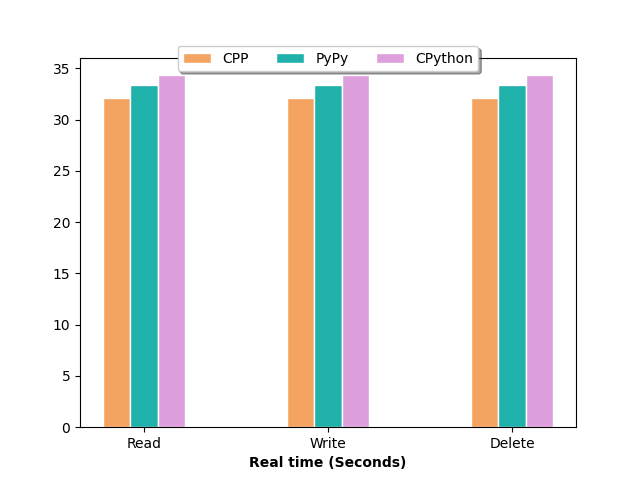
\includegraphics[width=7.5cm]{figures/real_time.png} }
    \subfigure{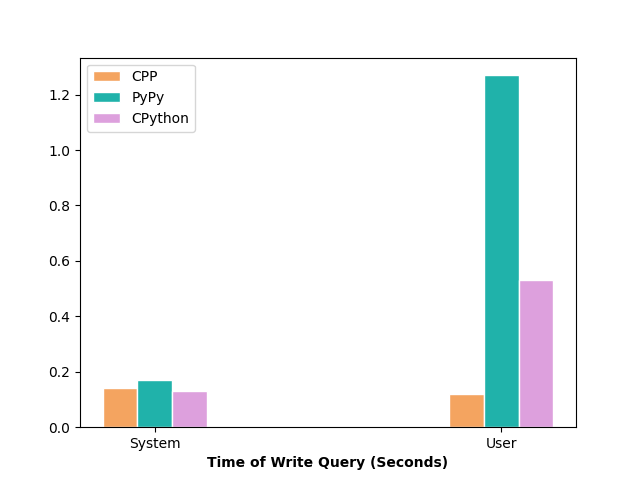
\includegraphics[width=7.5cm]{figures/time_user_sys.png} }
\end{figure}

As mentioned above, the left chart clearly shows that the client program has a significant network communication overhead and regularly waits for network interactions without using much CPU time.

\subsubsection{Profiling - CPU Usage}
The client program does not have a heavy computational overhead, and the chart below presents its CPU usage. The client CPU usage averages to 0\% for the compiled C++ program, while for PyPy, it is moderately higher, at 3\%.

\begin{figure}[H]
    \centering
    \subfigure{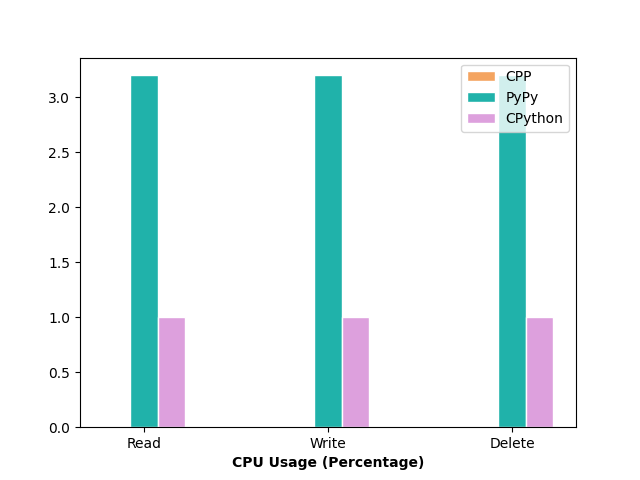
\includegraphics[width=7.5cm]{figures/cpu.png} }
\end{figure}

\subsubsection{Profiling - Memory Usage}
As shown in the memory usage charts below, PyPy uses more memory than CPython and C++. We speculate that this is due to two main reasons. First, CPython uses a garbage collector based on reference counting, and in C++ the objects are manually deallocated. In contrast, PyPy uses a hybrid garbage collection algorithm--it uses a nursery for the young objects and mark-and-sweep for the old objects.

The chart on the right presents the number of minor page faults. We speculate that the number of minor page faults in CPython is lower than PyPy because the reference counting GC algorithm can preserve the locality of the object references in memory.

\begin{figure}[H]
    \subfigure{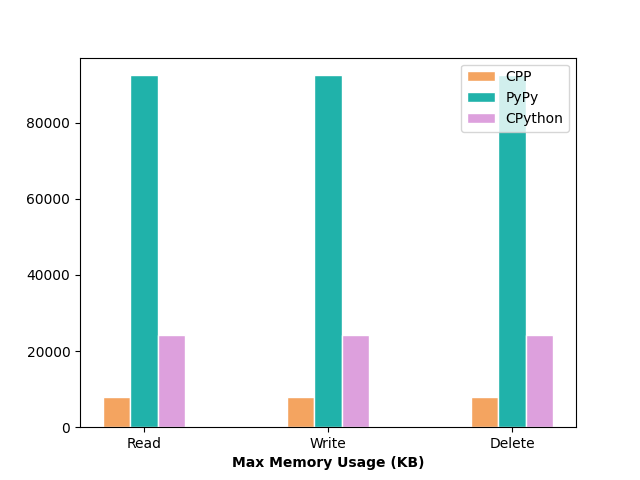
\includegraphics[width=7.5cm]{figures/max_memory.png} }
    \subfigure{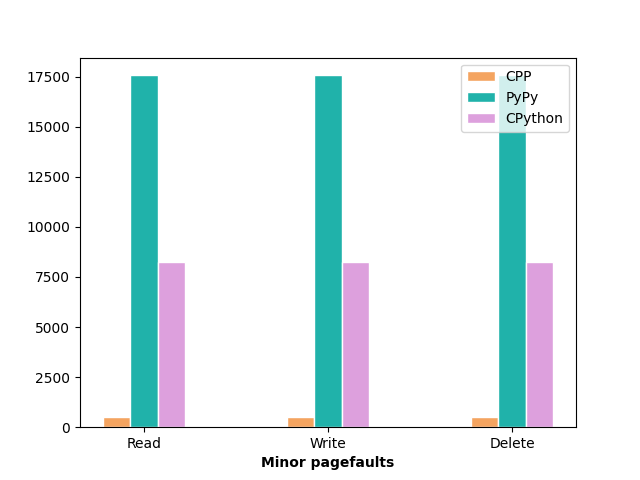
\includegraphics[width=7.5cm]{figures/minor_pagefault.png} }
\end{figure}
